% This is "sig-alternate.tex" V1.9 April 2009
% This file should be compiled with V2.4 of "sig-alternate.cls" April 2009
%
% This example file demonstrates the use of the 'sig-alternate.cls'
% V2.4 LaTeX2e document class file. It is for those submitting
% articles to ACM Conference Proceedings WHO DO NOT WISH TO
% STRICTLY ADHERE TO THE SIGS (PUBS-BOARD-ENDORSED) STYLE.
% The 'sig-alternate.cls' file will produce a similar-looking,
% albeit, 'tighter' paper resulting in, invariably, fewer pages.
%
% ----------------------------------------------------------------------------------------------------------------
% This .tex file (and associated .cls V2.4) produces:
%       1) The Permission Statement
%       2) The Conference (location) Info information
%       3) The Copyright Line with ACM data
%       4) NO page numbers
%
% as against the acm_proc_article-sp.cls file which
% DOES NOT produce 1) thru' 3) above.
%
% Using 'sig-alternate.cls' you have control, however, from within
% the source .tex file, over both the CopyrightYear
% (defaulted to 200X) and the ACM Copyright Data
% (defaulted to X-XXXXX-XX-X/XX/XX).
% e.g.
% \CopyrightYear{2007} will cause 2007 to appear in the copyright line.
% \crdata{0-12345-67-8/90/12} will cause 0-12345-67-8/90/12 to appear in the copyright line.
%
% ---------------------------------------------------------------------------------------------------------------
% This .tex source is an example which *does* use
% the .bib file (from which the .bbl file % is produced).
% REMEMBER HOWEVER: After having produced the .bbl file,
% and prior to final submission, you *NEED* to 'insert'
% your .bbl file into your source .tex file so as to provide
% ONE 'self-contained' source file.
%
% ================= IF YOU HAVE QUESTIONS =======================
% Questions regarding the SIGS styles, SIGS policies and
% procedures, Conferences etc. should be sent to
% Adrienne Griscti (griscti@acm.org)
%
% Technical questions _only_ to
% Gerald Murray (murray@hq.acm.org)
% ===============================================================
%
% For tracking purposes - this is V1.9 - April 2009

\documentclass{sig-alternate}

\begin{document}
%
% --- Author Metadata here ---
\conferenceinfo{Data-Intensive Computing for Text Analysis}{Fall 2011, School of Information, University of Texas at Austin}
\CopyrightYear{2011} % Allows default copyright year (20XX) to be over-ridden - IF NEED BE.
\crdata{0-12345-67-8/90/01}  % Allows default copyright data (0-89791-88-6/97/05) to be over-ridden - IF NEED BE.
% --- End of Author Metadata ---

\title{Meme Tracking in Scale with MapReduce}% \titlenote{(Produces the permission block, and
%copyright information). For use with
%SIG-ALTERNATE.CLS. Supported by ACM.}}
%\subtitle{Progress Report}
%\titlenote{A full version of this paper is available as
%\textit{Author's Guide to Preparing ACM SIG Proceedings Using
%\LaTeX$2_\epsilon$\ and BibTeX} at
%\texttt{www.acm.org/eaddress.htm}}}
%
% You need the command \numberofauthors to handle the 'placement
% and alignment' of the authors beneath the title.
%
% For aesthetic reasons, we recommend 'three authors at a time'
% i.e. three 'name/affiliation blocks' be placed beneath the title.
%
% NOTE: You are NOT restricted in how many 'rows' of
% "name/affiliations" may appear. We just ask that you restrict
% the number of 'columns' to three.
%
% Because of the available 'opening page real-estate'
% we ask you to refrain from putting more than six authors
% (two rows with three columns) beneath the article title.
% More than six makes the first-page appear very cluttered indeed.
%
% Use the \alignauthor commands to handle the names
% and affiliations for an 'aesthetic maximum' of six authors.
% Add names, affiliations, addresses for
% the seventh etc. author(s) as the argument for the
% \additionalauthors command.
% These 'additional authors' will be output/set for you
% without further effort on your part as the last section in
% the body of your article BEFORE References or any Appendices.

\numberofauthors{3} %  in this sample file, there are a *total*
% of EIGHT authors. SIX appear on the 'first-page' (for formatting
% reasons) and the remaining two appear in the \additionalauthors section.
%
\author{
% You can go ahead and credit any number of authors here,
% e.g. one 'row of three' or two rows (consisting of one row of three
% and a second row of one, two or three).
%
% The command \alignauthor (no curly braces needed) should
% precede each author name, affiliation/snail-mail address and
% e-mail address. Additionally, tag each line of
% affiliation/address with \affaddr, and tag the
% e-mail address with \email.
%
% 1st. author
\alignauthor
Hohyon Ryu\\
       \affaddr{School of Information}\\
       \affaddr{University of Texas at Austin}\\
       \email{hohyon@utexas.edu}
\alignauthor
Jae Hyeon Bae\\
       \affaddr{Computer Science}\\
       \affaddr{University of Texas at Austin}\\
       \email{metacret@gmail.com}
\alignauthor
Nicholas Woodward\\
       \affaddr{School of Information}\\
       \affaddr{University of Texas at Austin}\\
       \email{woodward.nicholas@gmail.com}
}

% There's nothing stopping you putting the seventh, eighth, etc.
% author on the opening page (as the 'third row') but we ask,
% for aesthetic reasons that you place these 'additional authors'
% in the \additional authors block, viz.
%\additionalauthors{Additional authors: John Smith (The Th{\o}rv{\"a}ld Group,
%email: {\texttt{jsmith@affiliation.org}}) and Julius P.~Kumquat
%(The Kumquat Consortium, email: {\texttt{jpkumquat@consortium.net}}).}
\date{09 December 2011}
% Just remember to make sure that the TOTAL number of authors
% is the number that will appear on the first page PLUS the
% number that will appear in the \additionalauthors section.

\maketitle
\begin{abstract}

With the recent development of Web 2.0 technologies and the concamitant explosion of user-generated content has come an incredible wealth of textual data whose form and content demand new strategies for text retrieval and classification.  In this paper we will describe our approach for extracting phrases that potentially allude to ideas, behaviors or styles that spread from person to person within a culture, collectively known as memes, from a large corpus of blog data.  In addition to phrase extraction, we use the canopy clustering approach \cite{McCallum2000} with a modified coefficent to group similar phrases.  Two Amazon Mechanical Turk\footnote{http://www.mturk.com} jobs are used to measure the likelihood that the clusters constitute a meme, and these data are used to build feature sets for supervising two support vector machines to classify the remaining clusters.

\end{abstract}

% A category with the (minimum) three required fields
\category{H.4.m}{Information Systems Applications}{Miscellaneous}
%A category including the fourth, optional field follows...
\category{H.5.4}{Information Interfaces and Presentation}{Hypertext/Hypermedia}

\terms{MapReduce, Blogosphere, Canopy Clustering, Amazon Mechanical Turk, SVM}

\keywords{Keyword Extraction, Data-intensive Processing, Implicit links in Blogosphere, Meme tracking}

\section{Introduction}

Web logs, also known as blogs, are a very important and interesting source of diverse information. They provide insight into the culture of the society in which they exist. People search blogs to find information on a their favorite interests or hobbies, to see what to do or where to go, and to discover what others think. Because blogs are typically written in plain language by individuals enthusiastic about particular topics, they may be more easily understood than longer, more-detailed news articles and cover a wider range of topics. Blogs are also more likely to contain memes, or ideas, behaviors and styles that are popular within a certain culture. Memes can generally be identified by relatively short, distinct phrases that travel from person to person in a society.  The fact that blogs are updated regularly makes them a good source for retrieving and extracting memes. 
//   In this study we experiment with a method for extracting, clustering and classifying memes from a large corpus of blog data.  Our approach builds on previous attempts at mining data from the blogosphere and more traditional text clustering and classification algorithms.  Additionally, we incorporate crowdsourced meme-ranking data obtained from Amazon's Mechanical Turk (MTurk) service to train our meme classifier.  The paper is structured as follows: Section 2 situates our project within the context of previous work.  Section 3 describes our approach to meme extraction.  Sections 4 and 5 discuss our methods of meme clustering and ranking, respectively.  Section 5 will review our evaluation method, and section 6 concludes with paper with a discussion of our results and some potential solutions to the challenges posed by research in the blogosphere.
\section{Related Work}
[blogs]
Retrieving them from a large collection of blog data presents several issues. [extend] 

Blogs are regularly updated they are highly sensitive to fast-changing temporal topics, finding and tracking memes, pieces of information that travel across blog posts, we can mine variety of issues and fads in the blogosphere. In this project we will extract memes from blogs, cluster them by their similarity, and rank the meme clusters using crowdsourcing-powered machine learning.
[text retrieval on the internet]

[text clustering and classifcation]

\section{Meme Extraction}

\subsection{Test Collection}

BLOGS08\footnote{http://ir.dcs.gla.ac.uk/test\_collections/blogs08info.html} is a TREC\footnote{http://trec.nist.gov/} test collection that crawled Web Logs from Jan/14/2008 to Feb/10/2009. It consists of 3 components: feeds, permalink documents, and homepage documents. We use only permalink documents that contain 28,488,766 documents and whose uncompressed size is 1445GB. 

\subsection{Preprocessing Blogs08}

Because the collection contains many duplicates, non-English blog posts, advertisement, and HTML tags, the following preprocessing is applied to Blogs08 collection using Python with Beautifulsoup, NLTK, and Decruft packages:

\begin{itemize}
\item Decruft
\item Removing non-English posts
\item Deduplication
\item HTML Strip
\end{itemize}


\subsubsection{Decruft}
Decruft\footnote{http://www.minvolai.com/blog/decruft-arc90s-readability-in-python/} extracts only meaningful content from a blog page, filtering out navigation links, advertisements, sidebar contents, and links to other sites. Decruft is a python implementation of ARC90's readability and it improves python-readability in terms of processing speed. 

\subsubsection{Removing non-English Posts}
We used NLTK\footnote{http://www.nltk.org/} language identification module to determine if the extracted content is written in English. After applying Decruft and removing non-English posts, extracted contents of a blog post are written into a single line per document for the MapReduce meme extraction process and the number of remaining posts was 166,749,81(96 GB).

\subsubsection{Deduplication}

Blogs08 also contains many duplicate documents and documents without significant amount of text. We set a lower-bound of 5 words and removed duplicates, also using Python. Finding duplicate document is $O(n^2)$, which requires tremendous amount of running time and computation. To improve its computational complexity and running time, we applied the following optimizations:

\begin{itemize}
\item First Character Indexing
\item Similar Length Indexing
\item Binary Vector of First 4 Characters of Terms
\end{itemize}

Instead of comparing against all other documents, binary vector of documents are stored in files named by the length of the vector and the lowercased first character of the document. Table \ref{table:dedup} shows an example of a blog post that is indexed in file 00030a. ``00030'' stands for the document length in terms of the number of unique words, and ``a'' stands for the lowercased first character of the document from ``At''. Ignoring HTML tags, the first 4 characters of all the words in the document are stored into the index file as a document vector. By using only first 4 characters, the vectors take less memory and disk space and computation for comparison becomes more efficient.


\begin{table}[h!t!]
\begin{center}
\begin{tabular}{l|p{6.0cm}}

\hline
DOC ID & BLOG08-20081015-016-0056752183\\ 

\hline
Document & 

At Work


\emph{(3 pictures omitted)}



(Photos: Zeitgeist Stage technicians take sand from the back alley of the BCA and spread it around the set for the current production of Seascape.)

Labels: At Work, Seascape, Zeitgeist Stage


- posted by Art @ 1:52 PM\\
\hline
File name& 00030a\\
\hline
Vector & and, set, curr, seas, back, at, art, alle, from, arou, for, 1, take, spre, prod, pm,labe, it, stag, post, by, phot, zeit, of, work, bca, 52, sand, tech, the\\

\hline
\end{tabular}
\caption{An example of the index for deduplication. The set of words are stored in a filed named concatenating the length of the word set and the lowercased first letter of the document.}
\label{table:dedup}
\end{center}
\end{table}


Once the vector generation is completed for all the documents, the deduplication program goes through the vector files, find duplicate vectors, and write a removal list which is a list of document ids that should be deleted in the next step. If a vector is shorter than 5, the document id is added to the removal list. The program nodes vector files of $\pm 2$ length of the current vector starting with the same character. Document simalarity is measures by the following formula:
\begin{displaymath}
dsim=\frac{A \cap B}  {min(|A|, |B|)}
\end{displaymath}

The denominator $min(|A|, |B|)$ was to give a tight denominator. A document that $dsim > 0.85$ with the current document was added to the removal list. In the third step, the entire collection is copied excluding the documents on the removal list. 1,570,428 documents (9.4\%) were removed leaving 15,104,553(85GB) documents after the deduplication process.

\subsubsection{HTML Strip}

Since this document collection will be used to present the blog post in a web interface, HTML tags were preserved. However, as meme extraction need only content text, a duplicate copy of the data collection  was created with HTML stripped and lowercased. The test collection for meme extraction became 43GB after stripping HTML tags with Python Beautifulsoup.




\subsection{Meme Extraction with MapReduce}

Preprocessed Blogs08 data is comprised of key-value pairs where the key is document number(doc\_id) and the value is the preprocessed content of the blog posts. Using Hadoop Streaming, Python MapReduce code extracts common phrases and groups documents by them. The overall algorithm design follows the algorithm presented in \cite{Kolak2008}. However, due to a scalability issue, lower bounds and upper bounds limit the output size of the data and the algorithms are simplified.  Additionally, our approach utilizes other optimizations such as stop word ratio check and preposition trimming. The three steps of MapReduce pseudo-code for Meme Extraction are illustrated in the following pseudo codes. The first MapReduce process splits the input text into sentences and extracts trigrams and their indices within the document. It checks if the trigram is comprised with only words. If all of the three words are stopwords according to a short stop word list shown in Table \ref{table:stopwords}, the trigram is ignored. The reducer removes the phrases($trigrams$) that appear less than 5 times or more than 300,000 times.

\begin{table}[h!t!]
\begin{center}
\begin{tabular}{p{1.5cm}|p {6.5cm}}

\hline

\hline
Short Stopword List & a, the, of, in, on, january, february, march, april, may, june, july, august, september, october, november, december, jan, feb, mar, apr, may, jun, jul, aug, sep, oct, nov, dec, am, pm \\
\hline
Long Stopword List & a, about, above, after, again, against, all, also, am, an, another, and, any, are, aren't, as, at, be, because, been, before, being, below, between, both, but, by, can't, cannot, could, couldn't, did, didn't, do, does, doesn't, doing, don't, down, during, each, few, for, from, further, had, hadn't, has, hasn't, have, haven't, having, he, he'd, he'll, he's, her, here, here's, hers, herself, him, himself, his, how, how's, i, i'd, i'll, i'm, i've, if, in, into, is, isn't, it, it's, its, itself, let's, me, more, most, mustn't, my, myself, no, nor, not, of, off, on, once, only, or, other, ought, our, ours , ourselves, already, out, over, own, same, shan't, she, she'd, she'll, she's, should, shouldn't, so, some, such, than, that, that's, the, their, theirs, them, themselves, then, there, there's, these, they, they'd, they'll, they're, they've, this, those, through, to, too, under, until, up, very, was, wasn't, we, we'd, we'll, we're, we've, were, weren't, what, what's, when, when's, where, where's, which, while, who, who's, whom, why, why's, with, won't, would, wouldn't, you, you'd, you'll, you're, you've, your, yours, yourself, yourselves, january, february, march, april, may, june, july, august, september, october, november, december, jan, feb, mar, apr, may, jun, jul, aug, sep, oct, nov, dec\\

\hline
\end{tabular}
\caption{Stop word list for blogs.}
\label{table:stopwords}
\end{center}
\end{table}

\begin{centering}

\begin{tabbing}
\textbf{MapReduce 1:}\\
\emph{Mapper 1:}\\

for \= ($doc\_id$, $text$) in [input file]:\\
\>	$sentences$  $\leftarrow$ split text by sentence boundary\\
\\
\>	for \= $sentence$ in $sentences$:\\
\>\>	$index$ $\leftarrow$ 0\\
\>\>	for \= $trigrams$ in $sentence$:\\
\>\>\>		$index$++	\\
\>\>\>		if \= checkStopwords($trigrams$)<1:	\\
\>\>\>\>		emit ($trigrams$, ($doc\_id$, $index$))\\
\\
\emph{Reducer 1:}\\
$lower\_bound$  $\leftarrow$ 5\\
$upper\_bound$  $\leftarrow$ 300000\\
for \= ($trigrams$, [($doc\_id$, $index$)]) in [mapper 1 output]:\\
\>	$len \leftarrow$ count([($doc\_id$, $index$)])\\
\> 	if \= $lower\_bound$ < $len$ < $upper\_bound$:\\
\>\>	emit ($trigrams$, [($doc\_id$, $index$)])\\
\end{tabbing}
\end{centering}

The second MapReduce process sorts the trigrams and indices by document to concatenate adjacent trigrams in MapReduce 3:

\begin{centering}
\begin{tabbing}
\textbf{MapReduce 2:}\\
\emph{Mapper 2:}\\
for \= ($trigrams$, [($doc\_id$, $index$)]) in [reducer 1 output]:\\
\>	for \= ($doc\_id$, $index$) in [($doc\_id$, $index$)]:\\
\>\> emit ($doc\_id$, ($trigrams$, $index$))\\
\\
\emph{Reducer 2:}\\
for \= ($doc\_id$, [($trigrams$, $index$)]) in [mapper 2 output]:\\
\>	emit ($doc\_id$, [($trigrams$, $index$)])

\end{tabbing}

\end{centering}

The third MapReduce process concatenates the adjacent trigrams within a blog post. Mapper 3 concatenates adjacent trigrams into a meme. Before emitting the memes a function trimPrepositions() removes prepositions at the beginning and end of the meme, and a function stopwordRate() checks how many of the words in the meme are stop words using the long stopword list shown in Table \ref{table:stopwords}. If stop words constitute more than 65\% of the words in the meme, the meme is ignored. In Reducer 3, phrases that are too short ($\leqq 5$) or too long ($\geqq 200$) are ignored as they are often timestamps, advertisement, or boiler plate text. The final MapReduce is illustrated as follows:

\begin{centering}
\begin{tabbing}
\textbf{MapReduce 3:}\\
\emph{Mapper 2:}\\

for \= ($doc\_id$, [($trigrams$, $index$)]) in [reducer 2 output]:\\
\>	$prev\_index=0$\\
\>	$meme=``"$\\
\>	for \= ($trigrams$, $index$) in [($trigrams$, $index$)]:\\
\>\>	if \= $index-prev\_index \leqq 3$:\\
\>\>\>		$meme$ += $trigrams$[3-($index-prev\_index$):]\\
\>\>	else:\\
\>\>\>		$meme$=trimPrepositions($meme$)\\
\>\>\>		if \= stopwordRate($meme$)<0.65:\\
\>\>\>\>		emit($meme$, $doc\_id$)\\
\>\>\>		$meme$=trimPrepositions($meme$)\\
\>\>\>		$meme$.append($meme$)\\
\>\>\>		$meme$=$trigram$\\
\>\>	$prev_index=index$\\
\\	
\>	\# clean up for the last one\\
\>		$meme$ = trimPrepositions ($memes$)\\
\>		if \= stopwordRate($meme$)<0.65:\\
\>\>		emit($meme$, $doc\_id$)\\
\\
\emph{Reducer 3:}\\
for \= ($meme$, [($doc\_id$)]) in [mapper 3 output]:\\
\> if \= $5 \leqq len(meme) \leqq 200$:\\
\>\>	emit ($meme$, [($doc\_id$)])

\end{tabbing}

\end{centering}

The final output is key, value pairs of a meme and the list of the document ids that the meme appears. In total, 4,610,100 memes are extracted from the TREC Blogs08 collection.

Table \ref{table:memeext} illustrates the parameters used for meme extraction.

\begin{table}[h!t!]
\begin{center}
\begin{tabular}{l|l}

\hline
\textbf{Parameter} & \textbf{Value}\\

\hline
Lowerbound for ngram appearance & 5\\
\hline
Upperbound for ngram appearance & 300,000\\
\hline
Lowerbound for meme length & 5\\
\hline
Upperbound for meme length & 200\\

\hline
Upperbound for stopword rate within a meme & 0.65\\

\hline
\end{tabular}
\caption{The parameters and optimizations used for deduplication.}
\label{table:memeext}
\end{center}
\end{table}

\section{Meme Clustering}

\subsection{Mahout LDA}
Latent Dirichlet Allocation (LDA)  characterize the document as the mixture of latent topics and the topic as the distribution of words \cite{Blei2003a}. LDA has shown significant improvement over previous attempts at topic modeling, most notably probabilistic latent semantic analysis \cite{Hofmann1999}.  It interprets each document as an unordered bag of words. Each word in the document is generated by first choosing the topic from topic distribution and then choosing the word from the word distribution, given the topic. When we denote the word, topic, document as $w, z, D$, the topic model formulates the following word distribution in the document:
\begin{displaymath}
 P(w)=\sum_{i=1}^K P(w|z_i)P(z_i)
\end{displaymath}
where $K$ is the number of topic for the corpus, $P(z_i)$ is the probability that $i$th topic was sampled for $w$, and $P(w|z_i)$ is the probability of $w$ given the $i$th topic. Using this interpretation, if we find the topic and word distribution for each document to maximize the probability of the entire corpus, we can group memes sharing similar sematical meaning.

Apache Mahout\footnote{http://mahout.apache.org} is the open source scalable machine learning library running based on Hadoop. It includes various machine learning algorithm for tasks such as  clustering, classification and recommender systems. Apache Mahout has an LDA implementation, but it has several drawbacks that led us to opt for a different solution in our study.

\subsubsection{Defect 1: Parameter estimation}
The primary issue with Mahout's LDA implementation is that it does not estimate parameters with variational Expectation Maximization (EM). In variational inference algorithm, the Dirichlet parameters $\alpha, \beta$ should be estimated to maximize likelihood of $p(\mathbf{w}|\alpha,\beta)$. Since a likelihood also is not tractable for computation, variational EM method should be used to maximize the lower bound of a likelihood value. But the Mahout LDA implementation does not estimate parameters and uses a fixed value submitted by the user on the command line as a $\alpha$ and log probability of a word given a topic as $\beta_{iw_n}$. We emailed the author of the implementation about the effects of parameter estimation, and he responded that it would not have much of an affect on the basic function of LDA. If we increase a topic smoothing parameter, it increases the effect of words that occur infrequently.

\subsubsection{Defect 2: Convergence}
The original LDA algorithm proposed the EM method to iterate until the lower bound of log likelihood value converged. The expectation step is an inference, and the maximization step is maximizing the lower bound of the log likelihood regarding the model parameters $\alpha, \beta$ using variational parameters obtained from the first step. The Mahout LDA implementation does not execute the maximization step and only repeats the expectation step using the previously calculated log probability of a word if given a topic.

\subsection{Yahoo! LDA}
Due to this limitation of the Mahout LDA implementation, we decided to use the Yahoo! LDA implementation\footnote{https://github.com/shravanmn/Yahoo\_LDA}. The Yahoo! LDA implementation is not based on Hadoop MapReduce, in part because of the limited programming paradigm of MapReduce and because its disk I/O between every job is not suitable for iterative machine learning representation. The Yahoo! Implemention of distributed LDA utilizes a message passing approach, as well as  Hadoop Streaming and HDFS (Hadoop Distributed File System) for job communication and intermediate shared storage. We attempted to run the Yahoo! LDA with our meme data collection on the Longhorn cluster at TACC, but all efforts were unsuccessful. Currently, the Yahoo! LDA implementation is operating with bash shell script for distributing work and synchronization, and we arrived at the conclusion that it is not fully equipped for a distributed environment. We encountered the following problems during our experiments:
\begin{itemize}
 \item Permission denied for excutables in jar package
 \item Synchronization problem of global/lda.dict.dump
 \item Ice::ConnectionLostException problem 
\end{itemize}
We were able to resolve the first two issues by modifying several lines of code in the script files, but we could not resolve the last problem. According to the Yahoo! LDA implementation author's email response, the lost connection problem is caused by Hadoop. The Yahoo! LDA implementation supports checkpointing and restart mechanisms, but when we attempted a restart the environment reverted back to what it was after the first iteration of LDA. The primary difficulty was the large scale of our collection (4 million memes), and many iterations were required to produce meaningful topic collection. On average each iteration ran for seven minutes with a single machine and 1.5 minutes with five machines. The default number of iterations of Yahoo! LDA implementation is 1,000.

\subsection{Mahout Canopy Clustering}
If we can represent our data as a vector, the most common and efficient clustering algorithm is $k$-means clustering. The main drawbacks of $k$-means clustering is that we have to specify the number of cluster $k$, a priori information of data distribution and $k$-means clustering is very sensitive to initial seed clusters. Thus, there are many suggestions that we can estimate suitable number of clusters and initial seed clusters using canopy clustering \cite{McCallum2000} because canopy clustering is generating clusters totally based on distance measure. Because Apache Mahout contains canopy clustering implementation, we implemented Jacadi distance measure to Apache Mahout interface and executed Mahout canopy clustering with some parameters.
\\   Canopy clustering receives 2 distance parameters $t_1, t_2$ such that $t_1 > t_2$. It starts with empty canopy list. If the distance between the vector and the canopy in the canopy list is less than $t_1$, the vector is added to the canopy. The distance from the canopy is the distance from the centroid of vectors in the canopy. If there is no canopy whose distance is less than $t_2$, which means the point is not strongly bounded for canopies, the new canopy is created with the point. This is repeated for every point.
We have more than 4.6 million memes and they are highly sparse. Without any tuning of canopy clustering algorithm, even though we specify very generous parameters for $t_1,t_2$, we would have more than million canopies it caused out of memory error while running on Hadoop MapReduce. Also, since its time complexity is near $O(N^2)$ with many canopies, we could not use the original canopy clustering implementation. After these trials and errors, we decided to develop Indexed MapReduce Canopy.

\subsection{Indexed MapReduce Canopy}
Since the form of memes evolve over time across different media \cite{Leskovec2009}, similar memes need to be clustered together. For example, ``lipstick look good on a pig," ``lipstick on the pig," and "lipstick on this pig" need to be seen in the same cluster. A canopy clustering algorithm \cite{McCallum2000} is used for this meme clustering. However, since we are clustering more than 4.6 million memes into many clusters of very fine granularity, different strategies should be adopted. Since Canopy is basically a single pass approach, the distance between every meme and every cluster needs to be calculated in $O(n^2)$ computational complexity. The meme clustering task is very different from an ordinary document clustering task as the number of documents is extremely high while the length of each document is usually fewer than a dozen of words. We devised the following optimizations and modifications to efficiently cluster 4.6 million memes:
\begin{itemize}
 \item Binary vector: A vector is simply a set of words in a meme or a centroid. The set operation is O(1) while list operation is O(n). Also word order is ignored by this method.
 \item Centroid indexing: The centroid is indexed by the words it includes so that when a meme is compared to only with the cluster centroids that include common words.
 \item New similarity coefficient: RBS similarity coefficient
 Jaccard's similarity coefficient 
\begin{displaymath} 
 J(A,B) = {{|A \cap B|}\over{|A \cup B|}}
\end{displaymath} 
  is not very suitable for our meme clustering as it is highly sensitive to the length difference between memes. We compare a meme with a cluster centroids, and when a cluster centroid is long, short memes cannot have high coefficient score and get assigned into any cluster. Therefore, we used a new coefficient named RBW coefficient. Instead of dividing by the union, we divide the number of common words by the average length of the two vectors to relieve the sensitivity:\\
\begin{displaymath}
RBW(A, B) = {{|A \cap B|} \over {(|A|+|B|) / 2} }
\end{displaymath}

Table \ref{table:sim} shows that Jaccardi's coefficient is much more sensitive to the length difference between a meme and a centroid. By dampening the sensitivity to the length difference, RBW coefficient is more sensitive to the intersection. 

\begin{table}[h!t!]
\begin{center}
\begin{tabular}{p{3.0cm}|p{2.2cm}|r|r}
\hline
\textbf{Meme}&\textbf{Centroid}&\textbf{Jaccardi}&\textbf{RBW}\\
\hline
weapons of mass destruction programs&&1.00&1.00\\
\hline
iraqs weapons of mass destruction & weapons mass destruction programs&0.60&0.75\\
\hline
fear of weapons of mass destruction & weapons mass destruction programs iraq&0.43&0.60\\
\hline
weapons of mass destruction and ballistic missiles&weapons mass destruction programs iraq fear&0.37&0.50\\
\hline
\end{tabular}
\caption{Comparison between Jaccardi's coefficient and the proposed RBW coefficient. Jaccardi's coefficient drops quickly as the centroid gets longer. On the other hand RBW coefficient is less sensitive to the length difference and more sensitive of the intersection.}
\label{table:sim}
\end{center}
\end{table}

The similarity score should be higher than 0.6 to be clustered into a given centroid.
 
 \item Stop word removal: The memes should be compared by meaningful words instead of stop words. Otherwise, ``You can put lipstick on a pig'' and ``You can put a book on the table" would be clustered together. Using an extended stop word list that includes month names and weekday names, we excluded stop words from the similarity computation. 
 \item Distributed computation: To cluster 4.6 millions of memes efficiently, mapreduce-based distributed Canopy approach, explained in Apache Mahout Canopy Clustering\footnote{https://cwiki.apache.org/MAHOUT/canopy-clustering.html}, is used. The mapper takes in a partial list of the memes. Using canopy algorithm, it generates cluster centroids. The reducer does the same clustering process with the aggregated centroids. The pseudo code of the MapReduce process is illustrated as follows:
 

\begin{centering}
\begin{tabbing}
\textbf{Meme-clustering:}\\
\emph{Mapper:}\\

$CIndex \leftarrow new HashMap$ \# Centroid Index\\
$C \leftarrow new List$ \# Cluster Centroids\\
for \= $meme$ in $memes$:\\
\>	\# Initialize $C$ and $CIndex$\\
\>	\# 0 is the index of the first cluster\\
\>	if \= $C$ is empty:\\
\>\>	\# set() makes a set of words in a meme\\
\>\>	$C$.append( set(meme) )\\
\>\>	for \= $word$ in $meme$:\\
\>\>\>		$CIndex$[$word$].add(0) \\
\\
\>	\# Get candidate centroids from $CIndex$\\
\>	$Candidates \leftarrow new Set()$\\
\>	for \= $word$ in $meme$:\\
\>\>		for \= $c$ in $CIndex$[$word$]:\\
\>\>\>		$Candidates$.add($c$)\\
\\
\>	$flag \leftarrow False$\\
\>	for \= $c$ in $Candidates$:\\
\>\>	if memeSim($meme$, $C$[$c$])>0.6:\\
\>\>\>		$C$[$c$]=$C$[$c$] + set($meme$)\\
\>\>\>	$flag \leftarrow True$\\
\>\>\>		for \= $word$ in $meme$:\\
\>\>\>\>		$CIndex$[$word$].add($c$) \\
\>\>\>		break
\\
\> if \= $flag == False$:\\
\>\>	$C$.append(set($meme$))\\
\>\>	$c$=len($C$)-1\\
\>\>		for \= $word$ in $meme$:\\
\>\>\>		$CIndex$[$word$].add($c$) \\
emit($C$)\\

\\
\emph{Reducer:}\\
\>The reducer is identical to the mapper except that \\
\> the input is the centroids($C$) instead of\\
\> the memes($memes$).\\

\end{tabbing}

\end{centering}

After the clustering, 2,010,355 cluster centroids were generated, and the 4.6 million extracted memes were assigned into these clusters.
 
\end{itemize}


\section{Meme Ranking}
Now that we have successfully clustered the memes, the task remains to classify them according to a meaningfulness or informativeness ranking. Though classification is a challenge, many of the meme clusters can easily be classified as meaningless because they contain sequences of words such as “2 1956 jamboree tues jan 3 1956 jamboree wed,oct 5th wed oct 4 tues” to do not form a coherent idea. If we extract some statistical features from meme clusters and build the training data indicating informativeness, we can predict informativeness of each meme cluster. Finally, if we build the model of classifier as a regression problem of probability of informativeness given a meme cluster, we can bring order into a set of meme clusters with the probability values. Currently, we are expecting the following features as discriminant to decide a meme cluster's informativeness.
\begin{itemize}
 \item the number of memes in the cluster
 \item average meme length
 \item average number of documents in the cluster
 \item average number of sources in the cluster
 \item meme cluster cohesiveness
 \item time span information of blog documents containing memes in the cluster
  \begin{itemize}
    \item the number of days blog documents were written
    \item the number of documents per day
  \end{itemize}
\end{itemize}
Meme cluster cohesiveness can be defined as 
\begin{displaymath}
\frac{the\ number\ of\ unique\ words}{the\ number\ of\ words}
\end{displaymath}
which means how similar memes in the cluster are each other.

\subsection{Building Training Set with Amazon Mechanical Turk}

\subsubsection{Initial Training Set (MT1)}
Ranking the meme clusters based upon their meaningfulness or informativeness as described above is a difficult and largely subjective task. Consequently, using machine learning for this task is highly problematic. To aid the process of automated classification of the phrase clusters, we implemented an Amazon Mechanical Turk (MTurk) to utilize human intelligence in building a training set \cite{Barr2006}. MTurk is an Internet service for scalable crowdsourcing of simple one-time tasks. It allows \emph{requesters} submit human intelligence tasks (HITs) to be completed by \emph{workers} in exchange for small payments. Requesters approve the results they consider satisfactory, and workers increase their confidence scores with high approval rates.

In our study, we displayed to the user a cluster of phrases and three 100-word snippets of text from the blog data in which the phrases appear, along with seven questions, or HITs, related to the meaningfulness of the phrases. Questions ranged from "Is this a meaningful chunk of information?" to "Is this a common expression that could potentially appear elsewhere?"  In total, we submitted 1090 meme clusters to MTurk with seven HITs each. Workers were required to have a HIT approval rate greater than 85\% and to have completed at least 50 approved HITs.
  All meme clusters were reviewed by three workers to allow for varying subjective assessments.  After removing the highest and lowest total scores to eliminate any individual biases, we calculated the mean score of the cluster and normalized on a 0-1 scale. Each meme cluster was then compared to a range of threshold values for the purposes of the Support Vector Machine, as described in the following section. The labels collected by this initial MTurk HIT is named Mechantal Turk Collection 1(MT1).

\subsubsection{Additional Training Set (MT2)}
Due to our limited success in classifying meme clusters using SVMs, we attempted another approach similar to the Bradley-Terry (1952) model for pairwise comparison.  For our second MTurk, we submitted 1,492 meme clusters to be compared sequentially by workers. After workers were presented with a definition for memes ("an idea, behavior or style that spreads from person to person within a culture") and examples of good and bad memes, workers were asked to select the better meme cluster. Meme cluster \#1 was compared to cluster \#2, cluster \#2 to cluster \#3 and so on. The labels collected by this pairwise comparison MTurk HIT is named Mechantal Turk Collection 2(MT2). The results were used to train the Bradley-Terry model, as described in the following section. 

\subsection{Ranking the Memes with Machine Learning Algorithms}
\subsubsection{Ranking with Supoprt Vector Machine}



From the result of the Mechanical Turk, we used 1090 meme clusters for training from MT1. The first method for meme ranking is classification using Support Vector Machine. Meme clusters in the training set were classified as positive or negative with the score threshold, and then we calculated the probability that a meme cluster in the training set is classified as the positive set. Sorting the meme clusters in the training set by the probability value allows us to find the most significant meme clusters. To do this we utilized the LIBSVM package\footnote{http://www.csie.ntu.edu.tw/$\sim$cjlin/libsvm/}. Our first task was to find the best threshold value to classify meme clusters in the training set as positive or negative. If a cluster's score is less than the threshold value then its class is negative.  Otherwise it is defined as positive. When we naively chose the threshold value as 0.5, our training data contained only 10\% negative data.   The trained model with this data predicted only 2 negative examples for the training set. As a result, we attempted several threshold values that could proved the best ratio of positive/negative data and prediction accuracy. Table \ref{table:svm} shows the results for several threshold values. We used the tool included LIBSVM package to find the best parameters and feature scale.

\begin{table*}[t!h]
\begin{center}
\begin{tabular}{c|p{3.5cm}|p{3.5cm}|p{3.5cm}|p{3.5cm}}

Threshold&No. of negative instances in training data&No. of negative instances predicted with the trained model&Cross-Validation accuracy(\%)&Training classification accuracy(\%)\\
\hline
0.5&108&2&90.2\%&90.2\% (984/1090)\\
0.6&321&4&70.8\%&70.9\% (773/1090)\\
0.7&427&38&61.3\%&62.1\% (677/1090)\\
0.75&587&577&56.2\%&72.8\% (794/1090)\\
0.8&639&1090&58.6\%&58.7\% (639/1090)\\
\end{tabular}
\caption{Classification experiment using SVM}
\label{table:svm}
\end{center}
\end{table*}

As we can see in Table \ref{table:svm}, the threshold value 0.75 appears to most adequately suit our needs, while the other values were unable to classify meme clusters as positive or negative. Using a threshold value of  0.75, we calculated the probability of positive classification for each meme cluster and then sorted the results. Figure \ref{fig:svm_result} shows the top 20 meme clusters.

\begin{figure}[h]
\begin{center}
\fbox{
\begin{tabular}{p{8cm}}

\begin{enumerate}
\item also offering a 500,are you offering senate candidate 2,offering 10,offering 1,offering 20,offering 30,offering 3,offering 4,offering 5,offering 6
\item am not 's design,decree of god,design to do's,god's decree,god's decree that those,god's design,it's design
\item 0 scientists,2004 scientists used,2008 scientists,400 scientists,january 2009 scientists have managed,the scientists used
\item 10 lessons,2008 lessons,2009 lessons,2 lessons,3 lessons,clarinet lessons 28,forgotten the lessons of 9
\item my own room happy memorable 2007,room 101,room 1,room 205,room 222,room 2,room 401,room 6,room 8
\item he's already gotten,he's gotten,it's gotten,she's gotten,that's gotten a lot of headline,what's gotten our shownotes,shownotes are complete,shownotes
\item 18 ct,1 slice,28 ct,32 ct,40 ct,6175 ne 195 ct,64 slice ct
\item it's sold,my soul's,sold at sotheby's,sold it's soul,s to be sold,the soul's,your soul's
\item energize a,energize,energize our,energize the,energize your,this would energize his supporters
\item a sultry,her sultry,sultry,the sultry,you are vixensexy and sultry
\item an exhortation,been my exhortation continually,exhortation,the exhortation
\item been snacking,be snacking,not too bad for snacking,snacking,while snacking
\item fear of rectum or,her rectum,his rectum,my rectum,the rectum,your rectum
\item cb,cb and so forth,cb,the cb
\item a centrist,conservative and centrist,more centrist,the centrist
\item it's required,required by today's,response to today's,that's required,what's required
\item a disgraceful,are disgraceful to ourselves,disgraceful,his disgraceful,offensive and disgraceful,the disgraceful
\item entitles him,entitles the holder,entitles them,entitles you
\item intimidate and terrorize,terrorize the,terrorize them,to terrorize
\end{enumerate}

\end{tabular}
}
\caption{Top 20 memes by SVM classification probability}
\label{fig:svm_result}
\end{center}
\end{figure}

Looking at the results, it is apparent that our approach is able to recognize several keywords or phrases in the meme clusters.  But this does not necessarily imply that those clusters are meaningful or informative in the same way as popular phrases that achieve critical mass. For example, if  we search for known memes such as  ``lipstick on a pig'' in the blog data the probability values of meme clusters containing this phrase are all less than 0.5, implying they are not meaningful or relevant. There are several potential causes for our results, including:
\begin{itemize}
 \item Errorneous feature engineering
 \item Reliability of Amazon Mechanical Turk training set
 \item Wrong approach to ranking the memes
\end{itemize}

Because evaluating feature engineering and training set is not easy, we try to rank meme clusters using regression method.



\subsubsection{Ranking with Support Vector Regression}
Regression is estimating the target value based on feature values. Instead of estimatimg probability of meme cluster to be informative, if we calculate scores using Support Vector Regression (SVR), to get informative meme clusters using the same training set from SVM experiment (MT1). We used $\epsilon$-SVR. Root Mean Square Error (RMSE) value for training set is 0.0171578, reasonable value. Figure \ref{fig:svr_result} is showing top 20 memes sorted by regression values.

\begin{figure}[h!b!p!]
\begin{center}
\fbox{
\begin{tabular}{p{8cm}}
\begin{enumerate}
\item carisoprodol carisoprodol,carisoprodol posted
\item bonnie and greta,greta
\item a chav,chav paderborn
\item despots and peons,despots
\item actions resulting,resulting actions
\item mysql usr,the usr
\item didn't budge,didn't burn
\item the eleusinian,the eleusinian mysteries
\item chilly powder,red chilly powder
\item a super old,super old
\item a major topic,major topic
\item altered nuclear transfer,nuclear transfer
\item i wantd,just wantd
\item degraw,sackett and degraw
\item the black strat,the strat
\item palatine ill,the palatine
\item johns house,taylor johns house
\item instant messaging systems,messaging systems
\item emil blonsky,soldier emil blonsky
\item diner dash 2,diner dash 1.106850
\end{enumerate}


\end{tabular}
}
\caption{Top 20 memes using Support Vector Regression}
\label{fig:svr_result}
\end{center}
\end{figure}

Unfortunately, this result does not look so informative either.

\subsubsection{Ranking with Pairwise Comparison}
In the final ranking approach we used a pairwise comparison, known as the Bradley-Terry model \cite{Bradley1952}. The model can be formulated by the following logit-linear form:
\begin{displaymath}
 logit[(P(i\ beats\ j)]=\lambda_i - \lambda_j
\end{displaymath}
where $\lambda_i=log\alpha_i$ for all $i$. If we assume that all comparisons are independent of each other, we can estimate $\lambda_i$ value with maximum likelihood estimate using a generalized linear model. In order to train the Bradley-Terry model, we used data from an MTurk of 1,492 meme pair comparisons from MT2. For each pair (A, B), we will have two training instances. If the evaluator decides A is better than B for the first instance, the class label is 1 and the features are difference of feature values from A to B. For another instance, a class label is -1 and features are difference from B to A. Using this evaluation approach with our training data, we learned the weights of different features using logistic regression. In this case, the bias should be always 0 because there are same number of instances in each class -1 and 1. Using the weights learned with this model, we can calculate the score of each meme cluster as a weighted sum of feature values. The results of this model, as shown in Figure \ref{fig:bt_result}, are superior to our results from ranking with support vector regression. In order to smooth the differences between feature values, we applied the $log$ function to the following features:
\begin{itemize}
 \item the number of memes in the cluster
 \item average meme length
 \item average number of documents in the cluster
 \item average number of sources in the cluster
 \item the number of days blog documents were written
\end{itemize}

\begin{figure}[!t]
\begin{center}
\fbox{
\begin{tabular}{p{8cm}}

\begin{enumerate}

\item they instruct the computer
\item ground of disfavored victimized by god
\item or other highly technological systems within their power
\item gods hate these
\item you grow and age it can create birth defects affect cellular development
\item asians into the united
\item expect etruscan strongholds
\item disfavored cities and the southern
\item a process of masculinization
\item the mediterreanean region is grossly disfavored
\item greed generate problems with money glorify overconsumption etc
\item 1492 exodus from spain spain became evil financed columbus initiated missionaries usa
\item centuries ago ruled with an iron fist
\item italian food creates fat people with stomach
\item be those whom traditionally maintained this type
\item gibralter broke through inundating the basin and killing untold
\item rich cultures helped the people understand and pursue lives
\item historical pattern and you will suffer for exploiting the
\item disfavored girls
\item i think these are the true candidates for immortality
\end{enumerate}
\end{tabular}
}
\caption{Top 20 memes using the Bradley-Terry model}
\label{fig:bt_result}
\end{center}
\end{figure}

Our original plan was training comparator with a binary classifier using Support Vector Machine. With the same training data described above, we can train the binary classifier for two instances. If we have two instances A, B, if A is better than B, the classifier has to return the label 1 for feature values of difference between A and B, otherwise -1. Armed with the accurate classifier, we can sort memes using the classifier as the comparator. But the problem was accuracy of classification. Training accuracy was slightly better than random, 59\%. The comparator has to return different labels for the difference from A to B and vice versa, but there are many cases the classifier is returning the same labels for each difference. With this inaccurate comparator, we cannot use this approach. Figure \ref{fig:bt_result} shows the top 20 memes that are ranked by Bradley-Terry model.

\section{Evaluation}

Context is essential to determine if a meme is informative and meaningful. If the meme ``lipstick on a pig'' is give without any context, it is just a phrase with a nonsensical meaning. However, it gains political meaning when it is provided in a full text: 
\begin{quote}
Let's just list this for a second. John McCain says he's about change, too, and so I guess his whole angle is, watch out, George Bush. Except for economic policy, health care policy, tax policy, education policy, foreign policy and Karl Rove style politics, we're really going to shake things up in Washington. That's not change - that's just calling the same thing something different. But you know, you can put \textbf{lipstick on a pig} - it's still a pig. (excerpted from BLOG08-20080916-022-0053659471 of TREC Blogs08 Collection)
\end{quote}

We built a web interface names Meme Browser(MB)\footnote{Available at http://stingray.ischool.utexas.edu/meme\_browser/} that highlights memes and provided related documents and timeline of a cluster of memes. Figure \ref{fig:mockup} shows an MB page that presents a blog post related to a meme cluster "lipstick on a pig." On top of the page, MB provides the histogram of the number of documents that included the memes in the same cluster. In this example, it is noticeable that the phrase "the lipstick on a pick" gained political connotation in September 2008, and frequently discussed throughout the month. The red bars below the time line histogram shows memes in the cluster and how long  and how many times those memes are mentioned in 2008 and early 2009. The histogram and the related memes support mouse over to provide detailed information as shown in the screen shot. Left left column of the central frame shows an article. With Decruft and CSS processing, only the contents are shown with a consistent format. The right column shows the list of blogs that the meme appeared. Using this interface, further evaluation will be done to determine the quality of extracted memes. MB help annotators to judge the meaningfulness of memes in context.

\begin{figure*}[h!]
	\begin{center}
		{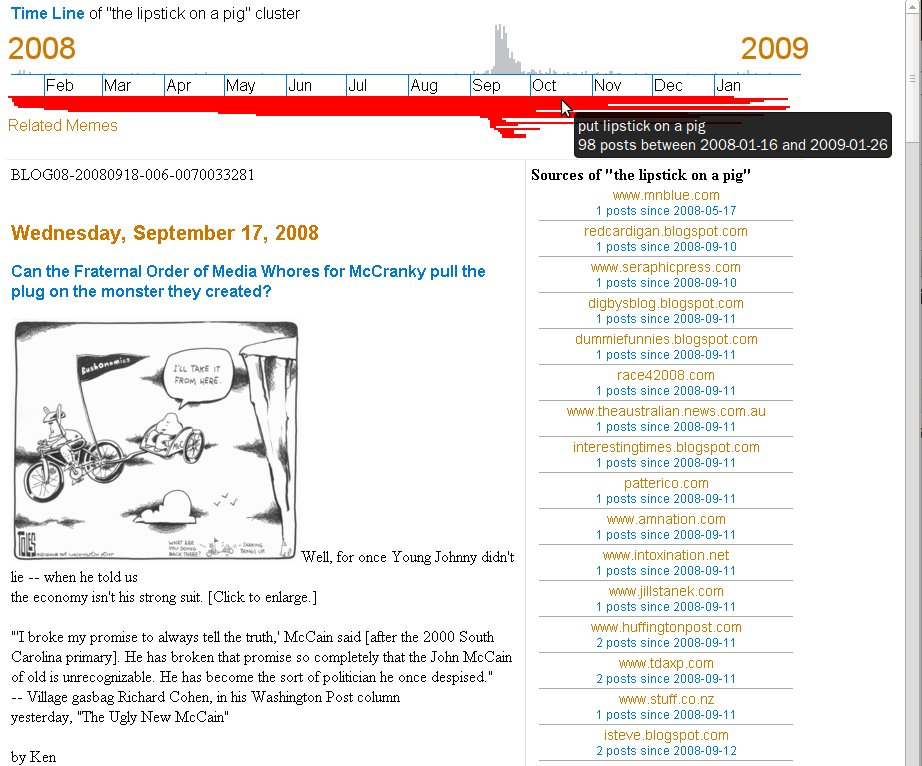
\includegraphics[width=\textwidth]{mockup.jpg}}
	\end{center}
	\caption{A Screen Capture of Meme Browser(MB).}
	\label{fig:mockup}
\end{figure*}

\section{Conclusion}
In this project, we used Hadoop MapReduce to discover informative memes from the large scale blog data. Differently from the previous topic discovery problem, we tried to discover fine-grained unit of information as denoted as \emph{meme} and evaluate them using machine learning technology and human intelligence through Amazon Mechanical Turk. In the process, we successfully completed challengeable text preprocessing tasks and devised a novel indexed approach for canopy clustering. We collected training data from Amazon Mechanical Turk and tried evaluation of meme clustering with a machine learning technology inspired by ''learning to rank``. The quality of this task is crucially dependent on not only laborous feature enginerring but also targeting appropriate machine learning framework. With the feature set, our classification and regression approaches did not work well, but we are approaching to discovery of informative memes with Bradley-Terry model. We believe that we can discover much information with more robust feature engineering and advanced machine learning technogy.

%
% The following two commands are all you need in the
% initial runs of your .tex file to
% produce the bibliography for the citations in your paper.
\bibliographystyle{abbrv}
\bibliography{sigproc}  % sigproc.bib is the name of the Bibliography in this case




\end{document}
